\documentclass[tikz]{standalone}
\usetikzlibrary{shapes.geometric, arrows.meta}

\tikzset{
    body/.style={draw, thick, fill opacity=0.5},
    dashed/.style={dash pattern=on 4pt off 2pt},
    bluebody/.style={body, draw=blue},
    orangebody/.style={body, draw=orange},
    blackbody/.style={body, draw=black}
}

\begin{document}
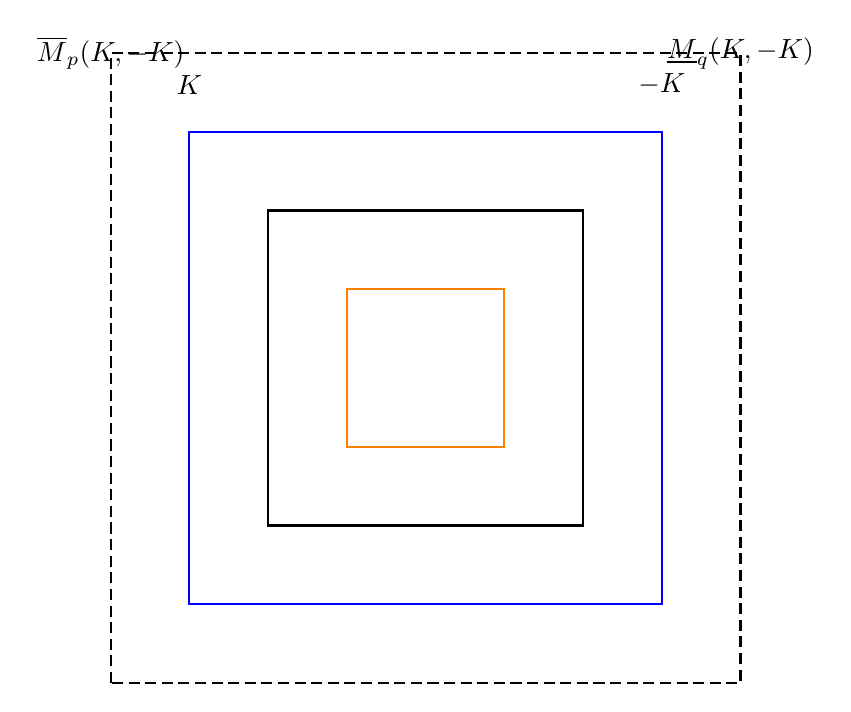
\begin{tikzpicture}[scale=2]

    % Draw K and -K
    \draw[blackbody] (-1, -1) rectangle (1, 1);
    \draw[dashed, blackbody] (-2, -2) rectangle (2, 2);

    % Draw M_p(K, -K)
    \draw[bluebody] (-1.5, -1.5) rectangle (1.5, 1.5);

    % Draw M_q(K, -K)
    \draw[orangebody] (-0.5, -0.5) rectangle (0.5, 0.5);

    % Labels
    \node at (-1.5, 1.8) {\(K\)};
    \node at (1.5, 1.8) {\(-K\)};
    \node at (-2, 2) {\(\overline{M}_p(K, -K)\)};
    \node at (2, 2) {\(\underline{M}_q(K, -K)\)};

\end{tikzpicture}
\end{document}